\section{System Implementation}

Among the related works in the previous section, a breadboard provides easy modification by its pluggable mechanism, and a piece of PCP offers fast wiring by printing out conductive ink. Thus, we present a new rapid prototyping tool, \papertitle, simultaneously adopting a pluggable and PCP fast wiring mechanisms.

\subsection{Hardware}

Since \cite{Instant_Inkjet_Circuits} presented a successful approach to inkjet printing circuits, we adopted a similar setup with a Brother DCP-J105 printer, silver nanoparticle ink NBSIJ--MU01, resin coated paper, and transparent PET film from Mitsubishi Paper Mill.

As illustrated in Figure X, \papertitle\ possesses a multi-layer design composing customized PCBs. Figure X is the top layer consisting of 10-by-30 female headers resembling the appearance and the pluggable mechanism of a breadboard. Figure X indicates the bottom layers where pieces of PCP are placed. The wiring on each piece of PCP determines the connections for the component pins on the top layer. Despite showing only X layers in Figure X, \papertitle\ can stack up to even more layers to create more connections which support more complicated circuits.

Each pin and contact pad in the center on both the top layer and the bottom layers connects to its corresponding pad on the sides. Each pad on the sides then contacts and electrically connects to its neighboring layers through a compressible on-board contact spring, part number OG-320816 (Figure X). Pads in the center on the bottom layers are also equipped with the same contact spring to push against the conductive ink on a PCP to form reliable physical contacts. Lastly, the layers and pieces of PCP are assembled and stacked up through tightening four screws on 4 corners.

\subsection{Software}

To create wire routing on PCP for \papertitle, the Breadboard tab in Fritzing \cite{Fritzing} functions as an interface (Figure X) for users to place components and arrange connections on a custom part, \papertitle. Then, the connection information in a Fritzing file, extracted through a Python script, is exported to a PCB design software, EAGLE \cite{EAGLE} where final connection arrangements and autoroute for PCP are created.


% \begin{figure}
%   \begin{center}
%   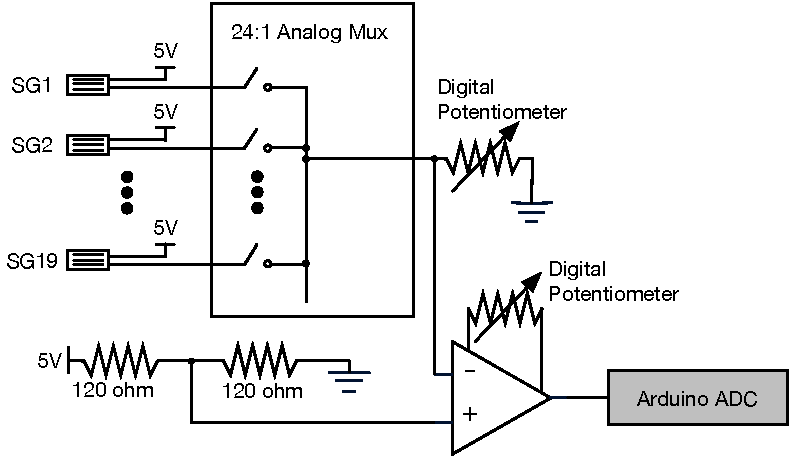
\includegraphics[width=1\columnwidth]{figures/Implementation.pdf}
%   \caption{The mechinical design of \papertitle }
%   \label{fig:FIGURE2}
%   \end{center}
% \end{figure}


% \begin{figure}
%   \begin{center}
%   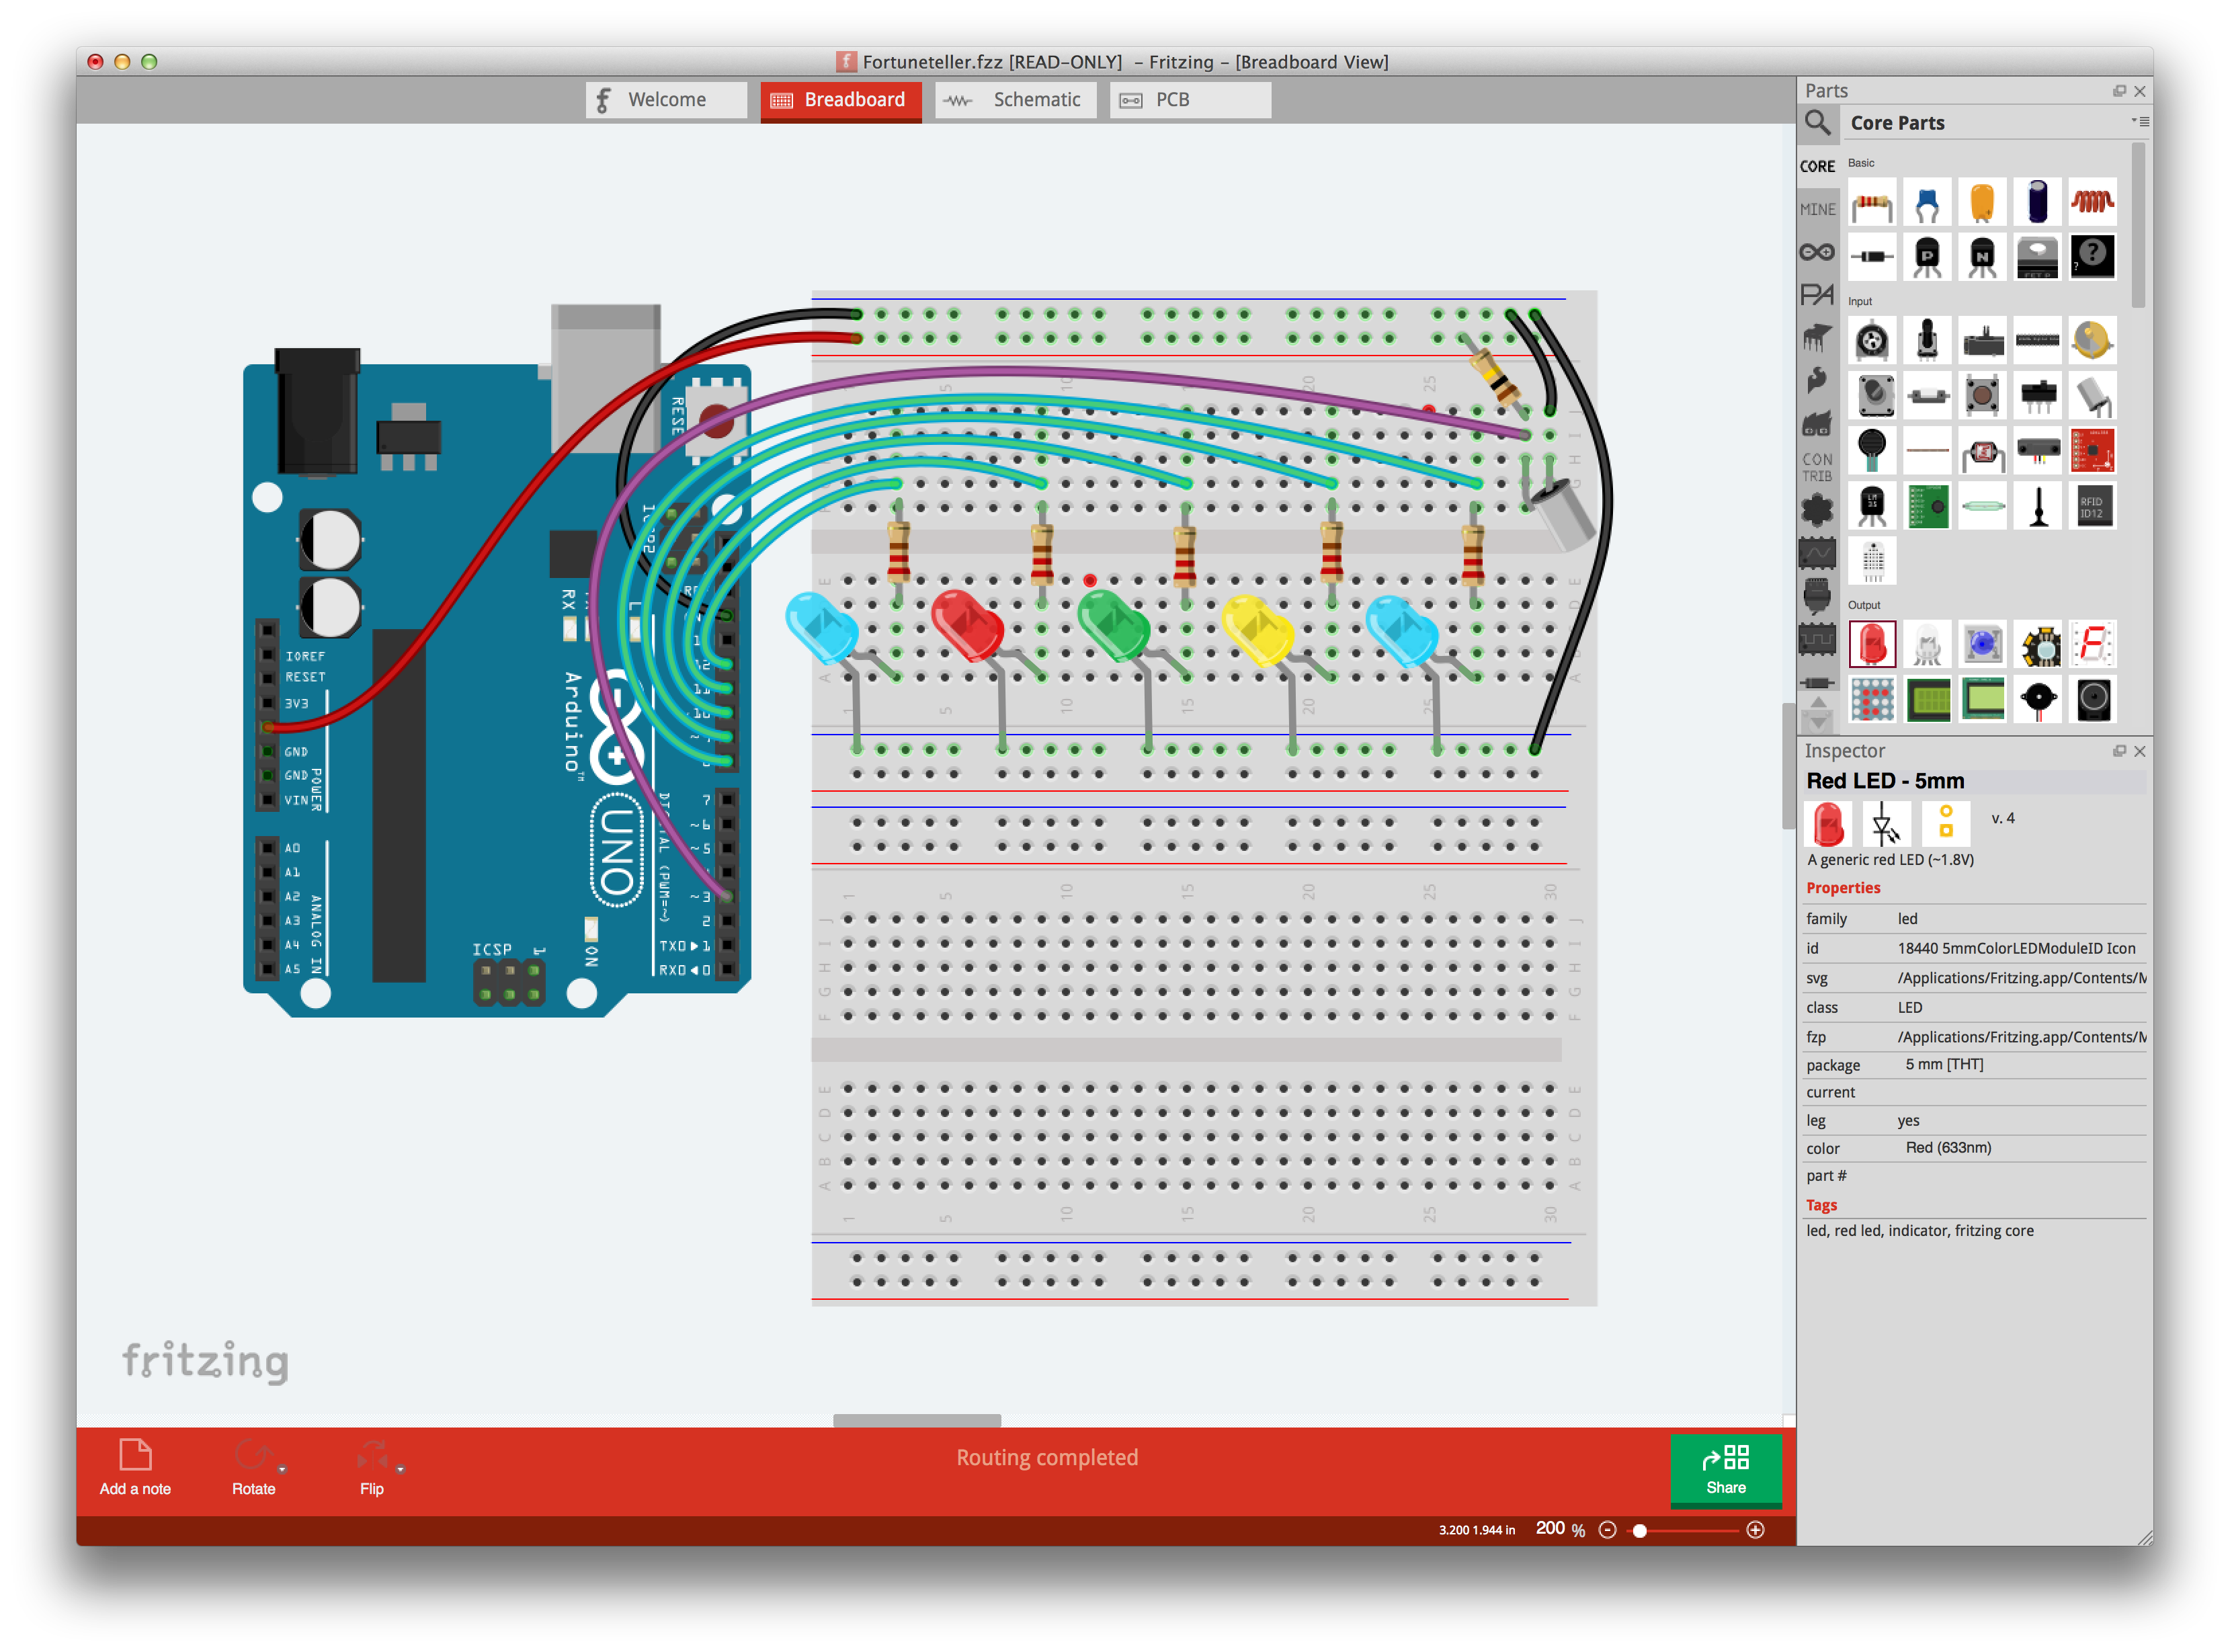
\includegraphics[width=1\columnwidth]{figures/GUI.png}
%   \caption{\papertitle also provides users a graphic user interface to help them design circuits efficiently.}
%   \label{fig:FIGURE4}
%   \end{center}
% \end{figure}
